
\section{JavaScript [R]}
Zuerst musste die Entscheidung gefällt werden, ob unser Projekt ein Standalone-Programm sein soll, oder im Browser zu erreichen ist. Weil wir aber wollten, dass es ein
Party-Game werden soll, dass man ohne jeglichen Aufwand sofort mit Freunden spielen kann, haben wir uns für die Browser-Variante entschieden.
Für mich war es eine leichte Entscheidung JavaScript zu verwenden, da die Programmiersprache genau für den Browser geeignet ist, und man damit nicht nur im Frontend, sondern auch im Backend programmieren kann.
\setauthor{Rafetseder Tobias}
\subsection{p5.js / p5.play [R]}
p5.js ist eine open-source JavaScript Library, die für Kreation von Spielen genutzt wird.
p5.play ist eine Library für p5.js, mit der man visuelle Objekte managen kann. Außerdem beinhaltet es Features wie Animation-support,
Kollisionserkennung, sowie aber auch Funktionen für Mouse und Tastatur Interaktionen.
Es ist wichtig sich im Hinterkopf zu behalten, dass p5.play für barrierefreies und simples Programmieren gedacht ist, nicht für perfomantes.
Es ist keine eigene Engine, und unterstütz auch keine 3D-Spiele.

\subsubsection{Einbindung}
Der einfachste Weg P5.js einzubinden ist auf ein JavaScript File online zu verweisen.

\begin{lstlisting}
    <script 
    src="https://cdn.jsdelivr.net/npm/p5@1.4.0/lib/p5.js">
    </script>
\end{lstlisting}
Man kann sich aber auch die P5.js Library
lokal downloaden unter \url{https://p5js.org/download/}
Dann muss man nur noch auf das lokale File verweisen.

\begin{lstlisting}
    <script src="../p5.min.js"></script>
\end{lstlisting}

Jedoch muss man das Projekt dann auf einem lokalen Server (z.B. Node.js) hosten.

\subsubsection{Struktur eines P5.js Projekts}
Die Struktur ist sehr simpel. Im Ganzen ist es nur ein \texttt{index.html} File und ein \texttt{sketch.js} File. In dem HTML File bindet man die P5 Library ein, und auch das sketch.js File.

\begin{figure}[H]
    \centering
    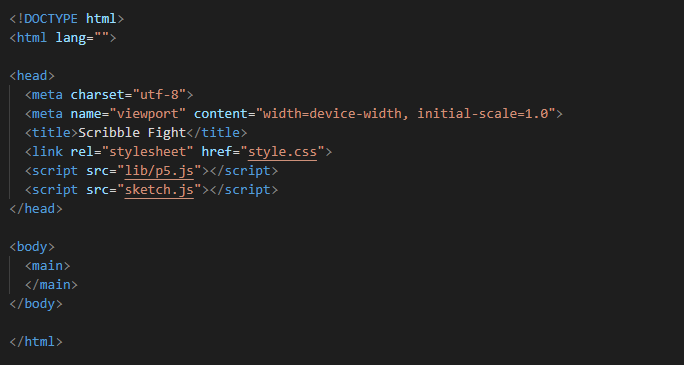
\includegraphics[scale=1]{pics/index html.PNG}
    \caption{Aufbau index.html}
\end{figure}

So kann man nun in dem sketch.js File die P5.js Methoden nutzen. Die wichtigsten Methoden sind die Setup- und die Draw-Methode.
Die Setup-Methode wird vor der Draw-Methode aufgerufen um das Spiel zu initialisieren. (Es wird zum Beispiel ein Canvas erstellt).
Wenn diese abgeschlossen ist, wird die Draw-Methode 60 mal in der Sekunde aufgerufen und updatet jedes mal den Bildschirm.

\begin{figure}[H]
    \centering
    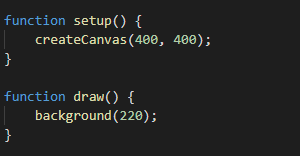
\includegraphics[scale=1]{pics/sketch.PNG}
    \caption{Simples sketch.js Beispiel}
\end{figure}

\subsubsection{P5.js vs Processing}
p5.js ähnelt sich sehr stark mit Processing, eine Programmiersprache die man sich wie ein stark vereinfachte Version von Java vorstellen kann.
Der Unterschied liegt darin, dass Java eine Umgebung, basierend auf der Java Programmiersprache ist, während p5.js eine Bibliothek, basierend auf der JavaScript Programmiersprache ist.
Processing ist dafür geeignet, lokale Applikationen zu bauen, hingegen dazu kann p5.js nur im Browser ausgeführt werden.

p5.js ist also kurzgesagt ein direkter JavaScript Port für die Processing Programmiersprache.

Vorteile von p5.js:
\begin{compactitem}
    \item Man kann interaktive Programme entwickeln, die in jedem modernen Browser funktionieren (plattformunabhängig)
    \item Das Programm ist nicht nur lokal auf dem eigenen Gerät, was das Teilen sehr viel leichter macht
    \item Man hat die Option den p5.js Editor im Web zu verwenden: Überhaupt kein Aufwand, um loszuprogrammieren
\end{compactitem}

Nachteile von p5.js:
\begin{compactitem}
    \item Ist langsamer beim Pixel manipulieren
    \item Ist kein Standalone-Programm, d.h. ein Browser wird benötigt
\end{compactitem}

\subsection {Node.js [R]}
Node.js ist eine plattformübergreifende Open-Source-JavaScript-Laufzeitumgebung, mit der Besonderheit, dass sie JavaScript-Code außerhalb eines Webbrowsers ausführen kann
und wurde ursprünglich von Ryan Dahl 2009 entwickelt, einem Software-Entwickler aus San Diego, Kalifornien.
Die Laufzeitumgebung wurde darauf spezialisiert, leicht skalierbare Server zu bauen.

In dem folgenden "Hello World"-Beispiel, können viele Verbindung gleichzeitig behandelt werden. Bei jeder Verbindung wird die Callback-Funktion ausgeführt, aber wenn keine Arbeit zu erledigen ist, schläft Node.js.

\begin{figure}[H]
    \centering
    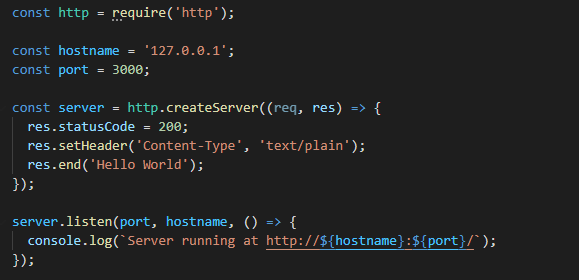
\includegraphics[scale=1]{pics/node js.PNG}
    \caption{Sehr simpler Node.js Server}
\end{figure}

Man merkt den Unterschied zu den heutzutage weit verbreiteten Concurrency-Modellen, die mit OS-Threads arbeiten. Der Vorteil von Node.js hierbei ist, dass
man sich keine Sorgen über dead-locking machen muss, da fast keine Node.js Funktion direkte I/O Operationen durchführt. Also ist der ganze Prozess so gut wie nie blockiert, ausser
wenn synchrone Methoden der Node.js Standard Library benutzt wird.

\subsubsection{NPM}
Neben Node an sich, ist NPM (Node Package Manager) das wichtigste Werkzeug für Node Applikationen. Mit NPM können alle Packages, die das Projekt benötigt, gefetched werden.
Es ist möglich, alle Packages einzeln zu fetchen, jedoch benutzt man normalerweise ein package.json File. In diesem File stehen alle Dependencies für jedes JavaScript Package,
das benötigt wird, sowie auch Meta-Daten zu dem Node Projekt. Erstellt wird dieses
in dem man in das Verzeichnis navigiert, in dem man das Projekt haben will und den Befehl \texttt{npm init} ausführt.

\begin{figure}[H]
    \centering
    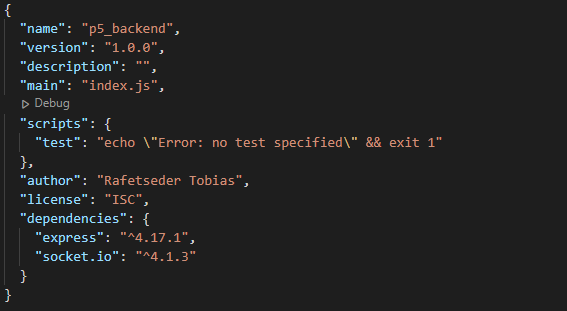
\includegraphics[scale=1]{pics/package json.PNG}
    \caption{Package.json des Scribble-Fight Backends}
\end{figure}

\subsubsection{Express}
Express ist das am meisten verbreiteteste Node Web Framework und ist auch die Basis für andere Node Web Frameworks. Die Hauptverantwortung
von Express ist das Bereitstellen von Server-Logik wie zum Beispiel das Schreiben von Handlers für Requests mit unterschiedlichen Http Verbs auf unterschiedlichen URL Pfaden.
Man kann Express mit dem Node Package Manager mit \texttt{npm install express} installieren, oder man befindet sich in
einem Verzeichnis mit package.json File bei dem Express als Dependency hinzugefügt wurde, dann reicht \texttt{npm install}

\begin{figure}[H]
    \centering
    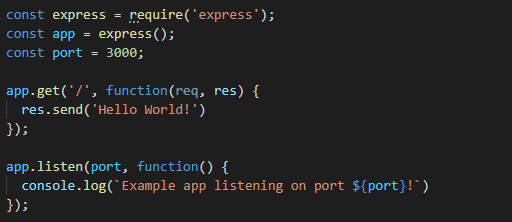
\includegraphics[scale=1]{pics/Express.PNG}
    \caption{Simpler Web Server mit Express}
\end{figure}

\subsection{Socket IO [R]}

Socket.IO ist eine Library, die eine bidirektionale Echt-Zeit Verbindung zwischen Server und Client ermöglicht. Es besteht aus
\begin{compactitem}
    \item Einem Node.js Server
    \item Einer JavaScript Client Library (Es bestehen auch einige andere Client Implementationen für Sprachen wie Java, C++, Python, etc.)
\end{compactitem}

Socket.IO funktioniert so, dass der Client, falls möglich, eine WebSocket Verbindung mit dem Server herstellt.
Ist keine Verbindung möglich, setzt der Client einen HTTP long polling Request ab.

\begin{figure}[H]
    \centering
    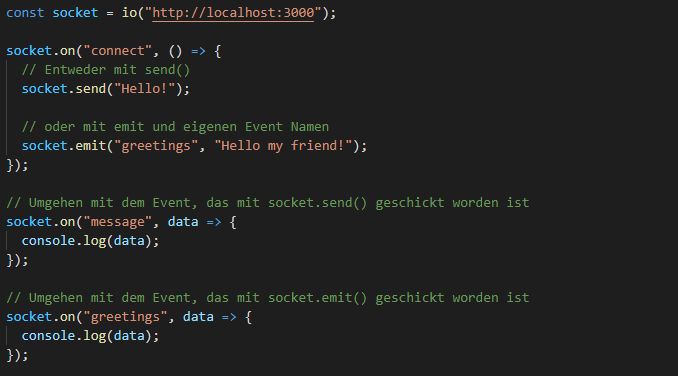
\includegraphics[scale=1]{pics/SocketIO_client.PNG}
    \caption{Socket.IO Client Beispiel}
\end{figure}

Damit der Server die Verbindung annehmen kann, müssen folgende Kriterien erfüllt sein:
\begin{compactitem}
    \item Der Browser unterstützt WebSocket
    \item Die Verbindung wird nicht von Elementen wie Firewall gestört
\end{compactitem}
Die API ist auf der Server-Seite dem Client sehr ähnlich, man bekommt auch wieder ein \texttt{socket} Objekt, welches von der EventEmitter Klasse von Node.js erbt.

\begin{figure}[H]
    \centering
    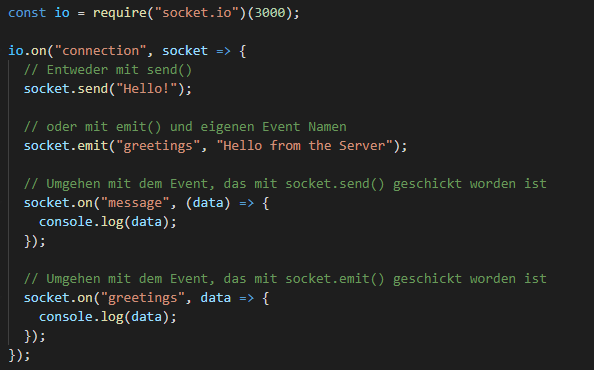
\includegraphics[scale=1]{pics/SocketIO_server.PNG}
    \caption{Socket.IO Server Beispiel}
\end{figure}


\subsubsection{Unterschied Socket.IO zu WebSocket}
Socket.IO ist keine WebSocket Implementation. Auch wenn Socket.IO WebSocket als Transportmittel benutzt, werden bei jedem Paket zusätzliche Metadaten angehängt. Das ist auch der Grund, warum
ein Socket.IO Client keine Verbindung mit einem schlichten WebSocket Server herstellen kann, und umgekehrt.
Man kann sich Socket.IO also als einen Wrapper rund um die WebSocket API vorstellen.

\section{Deployment [R]}
Das Scribble-Fight Browser-Game wurde in die Leocloud, ein Cloud-System der HTL-Leonding, unter \url{https://student.cloud.htl-leonding.ac.at/t.rafetseder/scribble-fight/} deployed.
Zuerst wurde mithilfe von der Docker-Technologie ein Docker-Image erstellt und auf die Leocloud hochgeladen. Das Deployment wurde dann mithilfe von Kubernetes umgesetzt.
Was Docker und Kubernetes genau ist, folgt in den nächsten Sektionen.
\subsection{Docker [R]}
Die Software Docker ist eine Technologie zum Containerisieren von Prozessen, die dann unabhängig voneinander und isoliert ausgeführt werden können. Diese isolierte Prozesse nennt man dann Container.
Durch die Unabhängigkeit, die dadurch entsteht, wird die Infrastruktur besser genutzt und auch die Sicherheit bewahrt, die sich aus der Arbeit mit voneinander getrennten System ergibt.
Docker arbeitet mit einem Image-basierten Bereitstellungsmodell. Dieses wird gerne bei Containertools verwendet, da Applikationen mit all deren Dependencies, egal in welcher Umgebung, genutzt werden können.
\begin{compactitem}
    \item Wenn man einmal seine containerisierte Applikation getestet hat, kann man sich sicher sein, dass die Applikation auf jeder anderen Umgebung, auf dem Docker installiert ist, auch funktioniert
    \item Alle Docker Container sind komplett voneinander unabhängig
    \item Falls Skalierung notwendig ist, kann man schnell neue Container erstellen
    \item Im Gegensatz zu virtuellen Maschinen beinhalten Container keine eigenen Operating Systems, deshalb kann man sie schneller erstellen und auch schneller starten
\end{compactitem}

Wichtige Begriffe, die man im Zusammenhang mit Docker kennen sollte:

\begin{compactitem}
    \item Image: Speicherabbild eines Containers
    \item Container: aktive Instanz eines Images
    \item Dockerfile: eine Textdatei, die den Aufbau des Images beschreibt
    \item Registry: Unter Registry versteht man eine Ansammlung gleicher Images mit verschiedenen Tags, meistens Versionen
\end{compactitem}

\subsubsection{Docker Architektur}
Die Docker Architektur ist eine Server-Client Architektur. Der Docker Client kommuniziert mit dem Docker Daemon, der dann Docker Container z.B. baut und ausführt.
Dieser Docker Daemon kann lokal installiert sein, aber der Client kann sich auch mit einem Daemon Remote verbinden.

\begin{figure}[H]
    \centering
    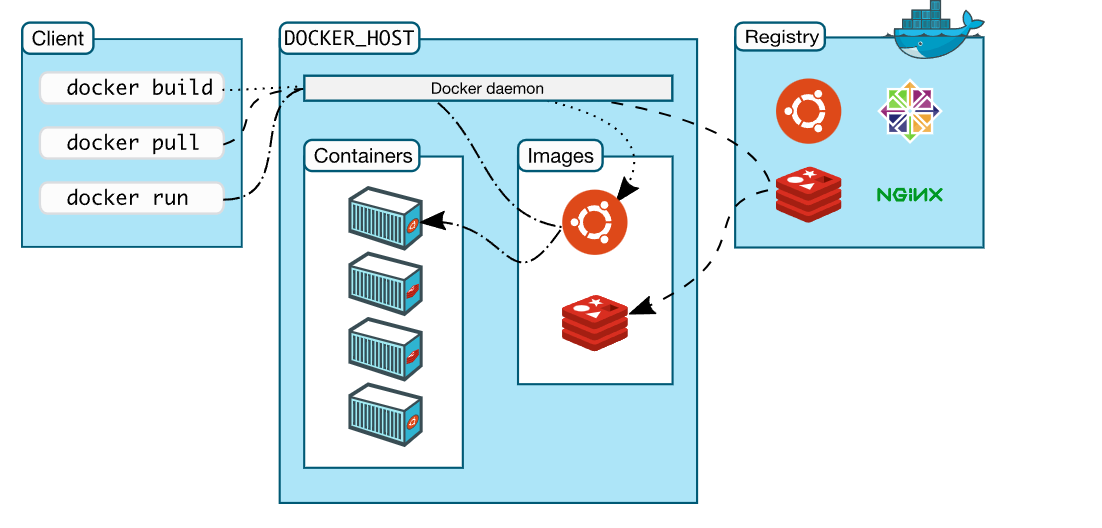
\includegraphics[scale=0.6]{pics/docker architecture.PNG}
    \caption{Veranschaulichung Docker Architektur}
\end{figure}


\subsection{Kubernetes [R]}
Kubernetes ist Open-Source-Plattform, die dafür genutzt wird, containerisierte Applikationen und Services zu verwalten. Es managed die Computer-, Netzwerk und Speicherinfrastruktur von Containern.
Das Kubernetes-Projekt ist 2014 als Open-Source Projekt in die Welt gerufen worden.

Kubernetes hat mehrere Funktionen, zum Beispiel ist Kubernetes:
\begin{compactitem}
    \item eine Containerplattform
    \item eine Microservices-Plattform
    \item eine Cloud-Plattform
\end{compactitem}

In dieser Diplomarbeit wird Kubernetes benutzt, um ein mit Docker gebautes Images des Scribble-Fight Browsergames auf ein Cloudsystem zu deployen. Näheres zur Umsetzung findet man \url{hier}

\newpage
\section{Python [H]}
Diese Programmiersprache, welche nach der Britischen comedy Serie ``Monty Python'' benannt ist,
fand in unserer Arbeit zwei Haupteinsatzgebiete. \\
Erstens, zur Erkennung des Blatt Papiers und der Umwandlung der Zeichnung in eine spielbare Map
und zweitens um die Künstliche Intelligenz zu erschaffen. \\
Die kostenlosen Bibliotheken, welche wir dabei in Verwendung haben, werden im folgenden gelistet und näher
erklärt.
\setauthor{Himmetsberger Jonas}

\subsection{Flask [H]}
Flask ist das am wohl häufigste verwendete Python Web-Framework. Somit gibt es viele Tutorials,
Tools und Bibliotheken. Diese sind sehr gut bis gut dokumentiert und teilweise geprüft.
Aus diesen Gründen haben wir den Teil der Bild- und Maperkennung, welche
als Webanwendung funktioniert, mittels Flask umgesetzt. In Kombination mit Flask-SocketIO werden Bilder von der Webcam
in Echtzeit direkt an den Server geschickt, welcher dann via OpenCV2 Informationen aus dem Bild
generiert. Genau wie bei SocketIO in JavaScript, agiert Flask-SocketIO als bidirektionale
Kommunikation zwischen Server und Client. Die extrem geringe Latenzzeit, welche dabei auftritt,
ist wichtig um eine flüssige Verarbeitung der Bilder zu gewährleisten.

\subsection{OpenCV2 [H]}
Open ``Computer Vision'' (CV) wurde in unserem Kontext als Python Bibliothek verwendet. OpenCV verfügt über eine
breitgefächerte Auswahl an Bildverarbeitungs-Algorithmen.
Folgende wurden bei der Maperkennung eingesetzt:
\begin{compactitem}
    \item Resizing
    \item Farbraumkonvertierung
    \item Weichzeichnung
    \begin{compactitem}
        \item Median-Blur
        \item Gaussian-Blur
    \end{compactitem}
    \item adaptive Schwellenwertbildung von Pixelwerten
    \item Konvertierung eines Zahlen Arrays in eine ``.png'' datei
\end{compactitem}
Auf die Funktionsweise dieser Algorithmen wird im Folgenden genauer eingegangen.
\\
Um zum Beispiel ein beliebiges Bild unscharf zu zeichnen würde man so vorgehen:
\\

\begin{lstlisting}[language=Python,caption=OpenCV Demo,label=lst:tech:gaussianBlur]
    # Dieses kurze Programm soll ein Bild in Python mittels Open Computer Vision weichzeichnen
    
    # Importieren der gebrauchten Bibliothek
    import cv2
    import numpy
    
    # Bild einlesen
    source = cv2.imread('./Pfad/zum/Bild.png', cv2.IMREAD_UNCHANGED)
    
    # Das Quell-Bild wird nun unscharf gezeichnet
    destination = cv2.GaussianBlur(source,(5,5),cv2.BORDER_DEFAULT)

    # Anzeigen von dem Quellbild und dem bearbeiteten Bild 
    cv2.imshow('Weichzeichnung',numpy.hstack((source, destination)))

    # warten, bis eine Taste gedrueckt wurde
    cv2.waitKey(0) 

    # Alle Fenster, welche die Bilder anzeigen, werden geschlossen
    cv2.destroyAllWindows() 
\end{lstlisting}

\subsection{PIL [H]}
PIL (Python Image Library) ist, wie Flask und OpenCV2, eine kostenlose Zusatzbibliothek für Python.
PIL wird verwendet um Bilder zu speichern und zu pixel zu manipulieren. Dabei unterstütz PIL diese
Dateiformate: PPM, PNG, JPEG, GIF, TIFF, und BMP. Pixel manipulation bedeutet, dass jeder Pixel auf einem
Input Bild angepasst werden kann. Beispiele hierfür sind zum Beispiel das Aufhellen oder Abdunkeln von
Bildern oder das Anpassen der Sättigung. Auch Kontrast- oder Schärfeeinstellungen können mit
Pixelmanipulation erzielt werden. Dafür werden meistens Matrizen und/oder Formeln pro Pixel verwendet um
deren Farbwerte anzupassen
\\



\begin{lstlisting}[language=Python,caption=PIL Demo,label=lst:tech:PIL]
    # verwendete Klassen der Bibliothek einbinden
    from PIL import Image, ImageFilter  

    source = Image.open("file.ppm") # Load an image from the file system.
    destination = source.filter(ImageFilter.BLUR) # Blur the image.

    # Display both images.
    original_image.show() 
    destination.show()
\end{lstlisting}



\subsection{TensorFlow und Keras [H]}
TensorFlow ist eine Python Bibliothek, welche beim erstellen von Projekten, welche maschinelles Lernen
in irgend einer Art und Weise eingebunden haben, extrem unterstütz.
Wie der Name schon vermuten lässt, basiert TensorFlow auf zwei Grundlagen: Tensoren und Graphen (Flow
vom Wort dataflow). \\
Tensoren sind besser bekannt als Skalare, Vektoren oder Matrizen. Tensoren sind also
null-, ein- oder mehrdimensionale Daten-Tupel.
TensorFlow bietet alles von on der effizienten Ausführung von
Befehlen auf der CPU, oder GPU, über der Skalierung von Berechnungen auf viele Endgeräte bis hin
zur Visualisierung der gelernten Daten mittels dem sogenannten ``TensorBoard''. TensorFlow ist also ein
sehr mächtiges Framework, das viele Möglichkeiten bietet, künstliche Intelligenzen zu trainieren und
analysieren.\\
Jedoch ist die Benutzerfreundlichkeit von TensorFlow sehr eingeschränkt. Viele Entwickler empfanden
es als ungeeignet für schnelles Prototyping und verwendeten daher das auf TensorFlow basierende Keras. \\
Keras verwendet standardmäßig die GPU zum ausführen von Code und is somit um einiges schneller als TensorFlow.
In dieser Diplomarbeit wurden zwei der von TensorFlow (Stable-Baselines3) bereits vorgefertigten Algorithmen,
namens ``A2C'' und ``PPO'', verwendet um die KI zu trainieren. Auf die Auswertung wird in \dots näher
eingegangen. Die Logik hinter der Künstlichen Intelligenz
wurde mittels OpenAI Gym implementiert.

\subsection{OpenAI Gym [H]}
OpenAI Gym ist ein Toolkit, mit welchem das Erlernen und Erstellen von reinforcement learning Algorithmen
sehr leicht fällt. Da viele Menschen nicht wissen, was ``reinforcement learning'' ist, wird es im folgenden
kurz erläutert.

\subsubsection{Reinforcement Learning[H]}
Reinforcement learning bedeutet auf deutsch so viel wie bestärkendes Lernen oder verstärkendes Lernen. Es
ist die dem biologischen Gehirn am nächsten Lernart.
Dabei basiert es auf folgendem Konzept: \\
Ein Agent, welcher etwas erlernen soll, wird in eine ihm unbekannte Umwelt gesetzt. Dieser kennt nicht mehr
als seinen eigenen Zustand und welche Aktionen er ausführen kann. Bewegt sich diese Entität nun in der
Umwelt, so passieren ihm Dinge. Diese können nach einer Observation entweder zu einer negative (-) oder einer
positive (+) Belohnung führen. Das einzige Ziel des Agenten besteht nun darin sein Tun so anzupassen, dass
er so viel und so
effizient wie möglich an diese Belohnung gelangt. Folgende Grafik erläutert das Beispiel an einem Hund,
welcher lernen soll einen Stecken zu apportieren.

\begin{figure}[H]
    \centering
    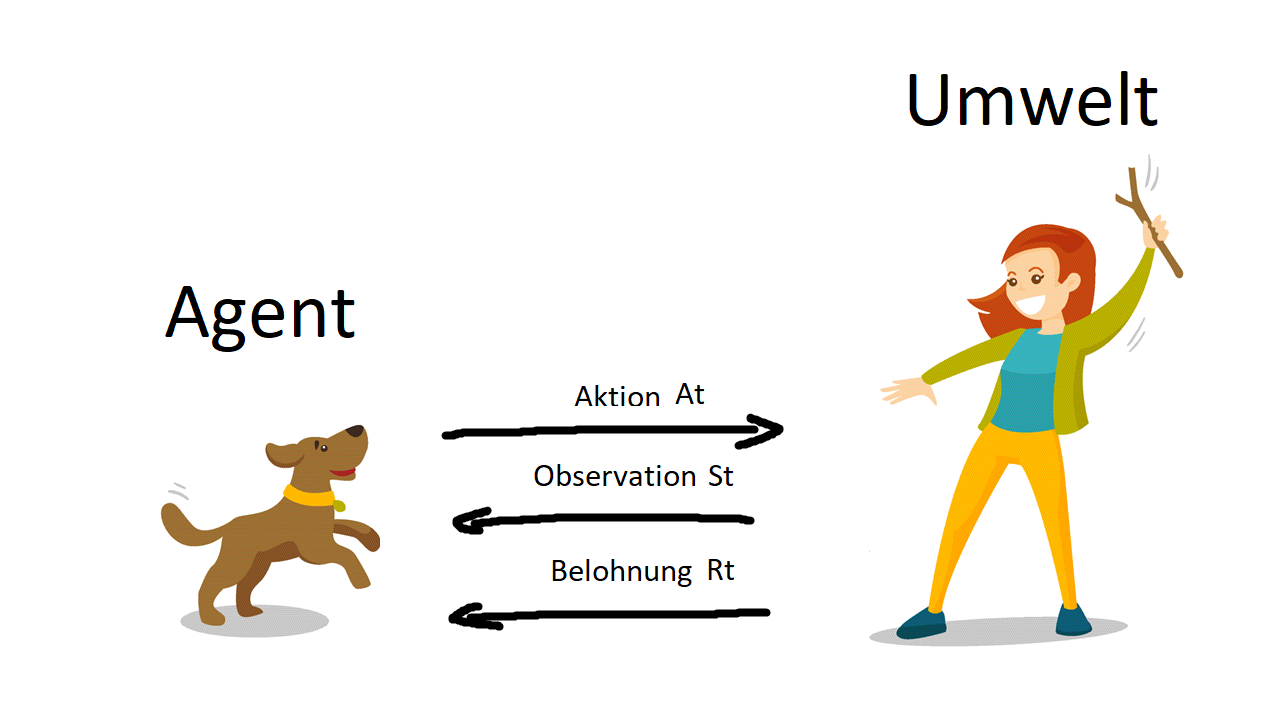
\includegraphics[scale=0.6]{pics/reinforcementLearningConcept.png}
    \caption{Veranschaulichung bestärkendes Lernen}
\end{figure}

OpenAI Gym hat also einen mehr oder weniger vorgegebenen Bauplan, und vorgegebene Regeln, nach welchen man
so eine Künstliche Intelligenz aufbauen muss. \\
Weitere, weit verbreitete Formen von machine learning sind supervised und unsupervised learning. Auf diese
wird nur weiter eingegangen, wenn zu wenig Text für eine positive Note für die Diplomarbeit vorliegen sollte.